\chapter{Mention2Vec Models}

In this chapter, we introduce two new multi-task models for POS and NER respectively. The multi-task model are based on the Mention2Vec model which is originally proposed for NER. We conduct experiments using the multi-task models on POS and NER and compare their performance and decoding speed with other neural network models.

\section{Model Description}

\subsection{Feedforward-Mention2Vec for NER}

Mention2Vec is a neural network model for NER, which uses BiLSTMs to predict boundaries and entity types separately (~\citeauthor{stratos2016mention2vec}, ~\citeyear{stratos2016mention2vec}). We summarize the Mention2Vec model into three steps. The first step is using a BiLSTM to generate hidden embeddings the same way in the BiLSTM-Char-CRF model. Figure \ref{fig:mention2vec1} illustrates the first step of Mention2Vec on a NER example. We denote the input sentence as $W: \left\{w_{1}, w_{2}, \dots, w_{n}\right\}$, vector concatenation operation as $\oplus$, input embedding as $X: \left\{x_{1}, x_{2}, \dots, x_{n}\right\}$ which are the concatenations of the character embeddings and the word embeddings, the hidden embeddings as $H: \left\{h_{1}, h_{2}, \dots, h_{n}\right\}$

\begin{figure}
  \centering
  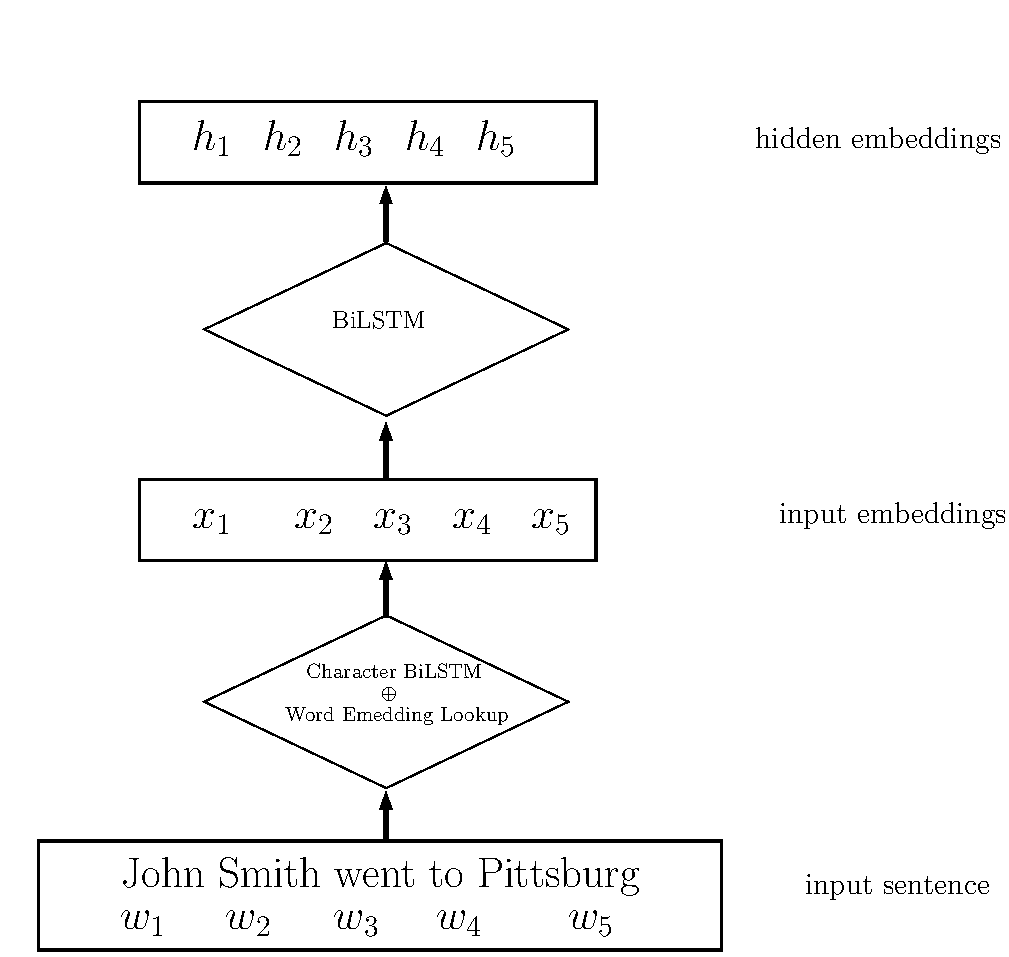
\includegraphics[scale=0.6]{mention2vec1.pdf}
 \caption{The first step of Mention2Vec for NER}
  \label{fig:mention2vec1}
\end{figure}

%In each training step, the model optimizes the boundary detection loss and type prediction loss jointly. We describe the Mention2Vec model for NER in detail here.
\begin{figure}
  \centering
  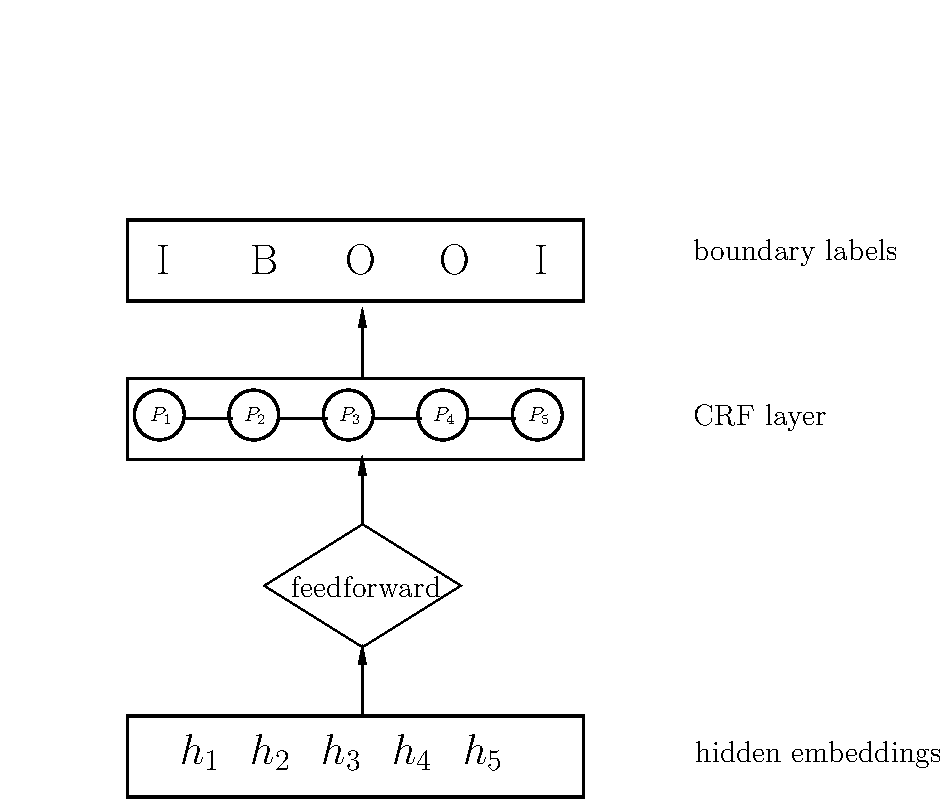
\includegraphics[scale=0.6]{mention2vec2.pdf}
 \caption{The second step of Mention2Vec for NER}
  \label{fig:mention2vec2}
\end{figure}

The second step of Mention2Vec is the boundary detection which is predicting $\left\{I, O, B\right\}$ labels for each word in a sequence. Unlike the usual NER labels (B-LOC, I-LOC, \dots), the boundary labels in this step do not have NER types attached. Mention2Vec takes the hidden embeddings produced in step 1, and feed them in to a feedforward network to get the boundary label probability distribution for each word. Since the boundary labels has strong correlations, Mention2Vec uses CRF to capture the correlations and produce the boundary label sequence. Figure \ref{fig:mention2vec2} illustrates the second step of Mention2Vec. The output boundary label probability distribution is denoted as $p_{i}$ for word $w_{i}$, and the gold boundary label sequence is denoted as $Y_{label}$. In each training step, the boundary detection loss is given by the negative log likelihood of the gold boundary label sequence, shown in \ref{eqn:loss1}

\begin{equation}\label{eqn:loss1}
  L_{1}\left(\theta _{1}\right) =-\log \left( p\left( Y_{label}|h_{1}, h_{2} \dots h_{n}\right) \right) 
\end{equation}

The third step of Mention2Vec is the type prediction which is finding the actual types for each named entity span in the sequence. It makes use of the hidden embeddings and the entity boundaries from the previous two steps. The model first looks up the hidden embeddings for the words in entity spans. Then, it feeds the word span hidden embeddings into an additional BiLSTM and obtains the corresponding vector representations for the word span $\mu$ by concatenating the final forward and the backward states produced by the BiLSTM. A feedforward network, at the end, is used to map the word span vector representations $\mu$ to type probability distributions. Figure \ref{fig:mention2vec3} illustrates the third step of Mention2Vec.

\begin{figure}
  \centering
  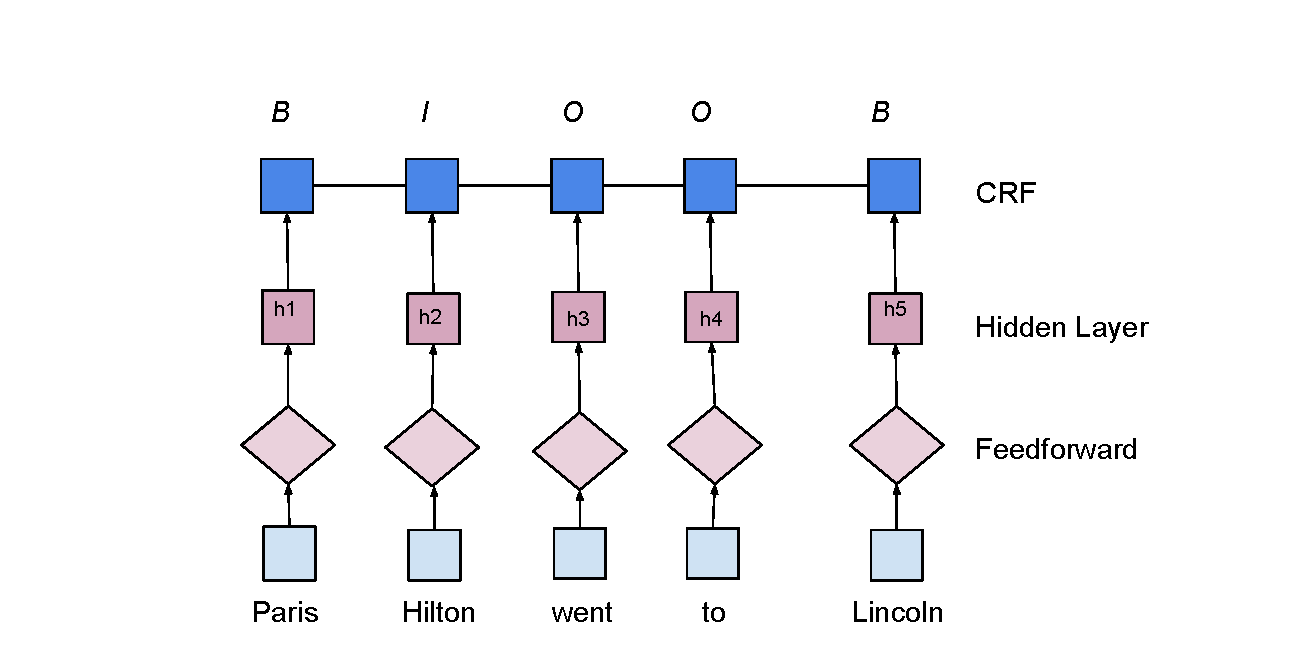
\includegraphics[scale=0.6]{mention2vec3.pdf}
 \caption{The third step of Mention2Vec for NER}
  \label{fig:mention2vec3}
\end{figure}

The gold type label sequence of an input sentence is denoted as $Y_{type}$. Assuming there are $l$ named entities in a sentence, and the index of the first word in a named entity is represented as $s$, and the index of the last word in a named entity is represented as $e$, the type prediction loss is computed by \ref{eqn:loss2}:

\begin{equation}\label{eqn:loss2}
  L_{2}\left(\theta _{2}\right) =-\sum _{l}\log P\left( r^{l}|h_{s}^{l}{\ldots }h_{e}^{l}\right)
\end{equation}

During training, the model uses the gold boundaries and gold types to compute the boundary detection and the type prediction loss. In each training step, the boundary detection loss and the type prediction loss are minimized jointly: the training objective is to find the boundary sequence and type sequence that minimize the sum of $L_{1}$ and $L_{2}$.


In order to further speed up the the tagging system as well as capture the correlation between boundary tags, we consider using a different network for boundary detection. Shown in Chapter 2 and Chapter 3, Feedforward-CRF produces relatively good performance on NER with faster speed than BiLSTM. We then replace the BiLSTM in the first step of Mention2Vec with a feedforward network. We denote this new model for NER as Feedforward-Mention2Vec. Feedforward-Mention2Vec still has three steps, the second step and the third step are the same as the ones in Mention2Vec. The first step uses a feedforward network to produce the hidden embeddings, which is illustrated in Figure \ref{fig:mention2vec4}.

\begin{figure}
  \centering
  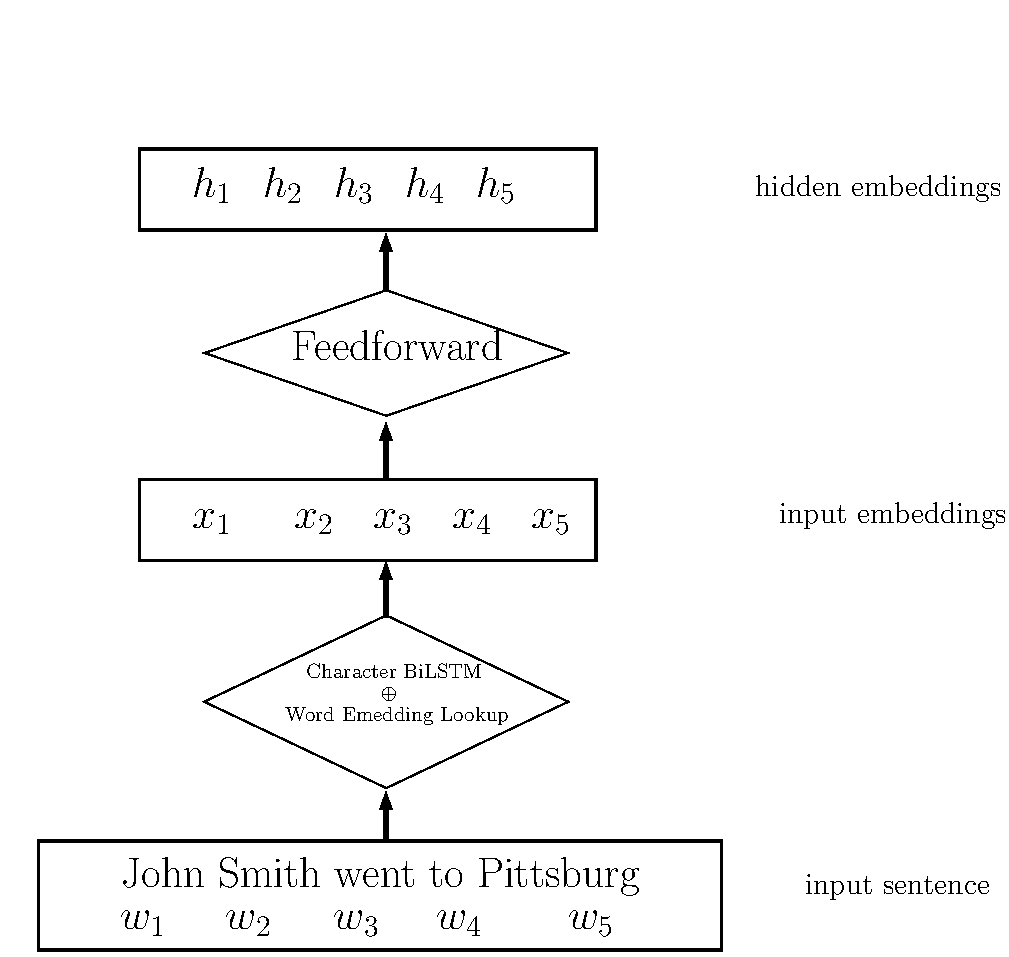
\includegraphics[scale=0.6]{mention2vec4.pdf}
 \caption{The first step of Feedforward-Mention2Vec for NER}
  \label{fig:mention2vec4}
\end{figure}

The run time of decoding the boundaries is constant in both Feedforward-Mention2Vec and Mention2Vec, since there are only three types of boundaries ("I", "O", "B") to decode in the CRF layer. In other CRF based models, like BiLSTM-Char-CRF, the decoding time grows quadratically in the number of named entity types. 

\subsection{BPE-Mention2Vec for POS}
In POS, each word in the input sentence is assigned a unique part-of-speech tag. Since there is no part-of-speech span existing in POS, it's not necessary to use a multi-task model on POS. However, we come up a way to convert POS into a NER-like task through the help of Byte Pair Encoding. Inspired by the successful results obtained by using BPE in machine translation (~\citeauthor{sennrich2015neural}, ~\citeyear{sennrich2015neural}), we initially wanted to use BPE to capture morphological decomposition of the words and replace spelling features like prefix and suffix. BPE is a compression algorithm which replaces frequent pairs with an unused byte. \cite{sennrich2015neural} presents a way to adapt BPE for word segmentation: using BPE to segment words into subword units of different length, and building a vocabulary dictionary using word frequency. In the POS tagging system, we first learn BPE merge operations on the training data. To segment training data and test data, we first split each word in characters and them apply BPE to merge the characters into larger chunks. In order to restore the words, we use the "IOB" label scheme to label the subword units. Since there can be multiple subword units sharing the same tag, POS becomes a task similar with NER. Figure \ref{fig:bpe} shows an example result after using BPE to segment a sequence with POS tags. 

In our proposed BPE-Mention2Vec model for POS, there are three main steps. In the first step, given a sequence, we use BPE to segment the words and convert the corresponding tags using the "IOB" label scheme. After the first step, we have a NER-like task with known boundary of each entity span, so we can apply the same methods in Feedforward-Mention2Vec to predict the POS types for entity spans. In the second step, we use a feedforward network to produce the hidden embeddings of the input words. CRF is not used here because that the boundary labels are known in both training and decoding. The third step of BPE-Mention2Vec uses a BiLSTM to predict the POS tags for each entity span based on the hidden embeddings and the known boundaries. Figure \ref{fig:bpemention2vec} describes the process of using BPE-Mention2Vec to find POS tags for a sequence. 


\begin{figure}
  \centering
  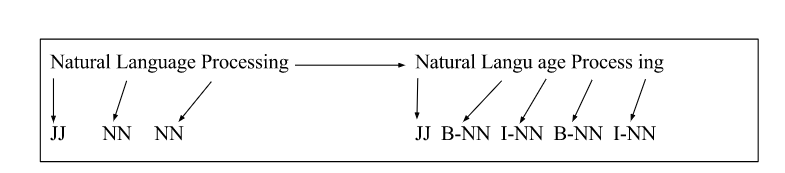
\includegraphics[scale=0.5]{bpe.png}
 \caption{An example of using BPE for word segmentation}
  \label{fig:bpe}
\end{figure}

\begin{figure}
  \centering
  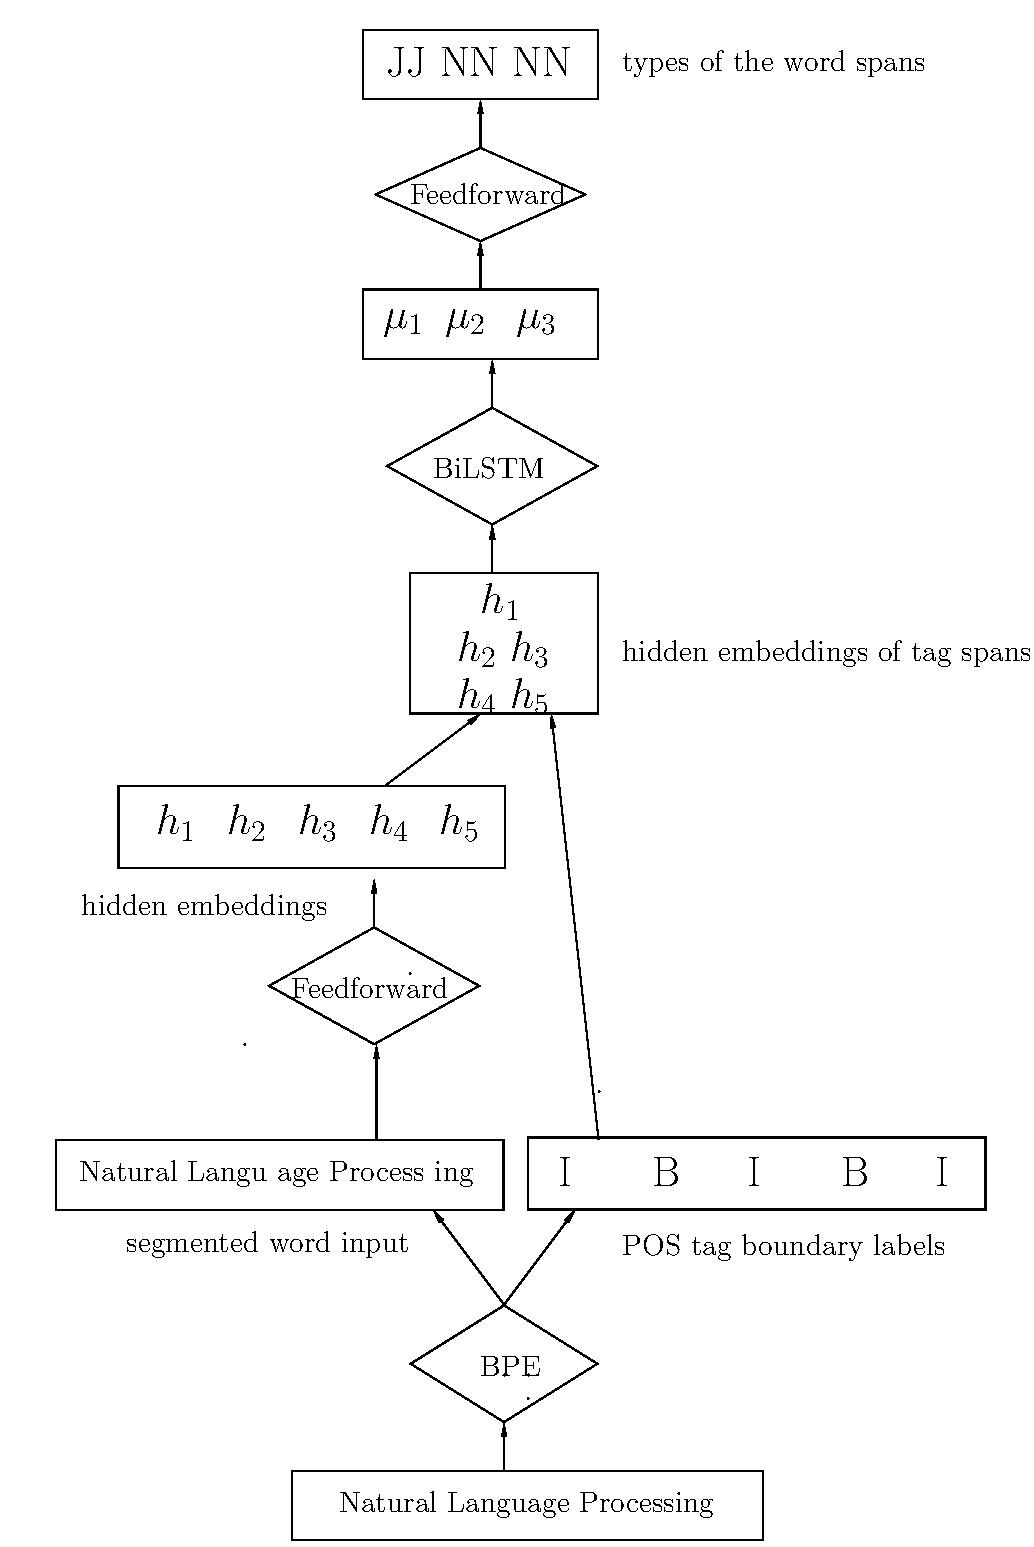
\includegraphics[scale=0.6]{bpemention2vec.pdf}
 \caption{An example of using BPE-Mention2Vec to find POS tags}
  \label{fig:bpemention2vec}
\end{figure}

\section{Experiments and Results}

We empirically evaluate the Mention2Vec model and the Feedforward-Mention2Vec model for NER, and the BPE-Mention2Vec model for POS. We implement these models in Python and Tensorflow 1.0. The experiments in this section use the same set of hyperparameters in the previous experiments. 

In the NER experiments, we compare the Feedforward-Mention2Vec model with the original Mention2Vec model on the CoNLL 2003 data set. We use the BiLSTM-Char-CRF model as the baseline model since it achieves the highest F1 score among the previous models we built, and it is recognized as the state-of-the-art model for NER. Table \ref{table:ner-mention2vec1} demonstrates the NER performance and decoding speed of these three neural network models on CoNLL 2003 data set. Mention2Vec achieves 89.51 F1 score which is lower then the 90.11 F1 score of BiLSTM-CRF, and it is slightly slower than BiLSTM-Char-CRF. Feedforward-Mention2Vec achieves 88.79 F1 score compared to 89.51 of Mention2Vec and 90.11 of BiLSTM-Char-CRF, but it is 1.4 times faster than Mention2Vec and 1.3 times faster than BiLSTM-Char-CRF. The empirical results demonstrate that the Feedforward-Mention2Vec model performs competitively on the CoNLL 2003 NER tagging task while being faster than original Mention2Vec model and the state-of-the-art model.

Since we have known that Feedforward-Mention2Vec and Mention2Vec scale linearly in the number of named entity types while BiLSTM-Char-CRF grows quadratically. We want to show the time difference of the same model on NER data sets with different numbers of named entity type. Now we have the performance and decoding speed of these models on CoNLL 2003 which has 4 types of named entity. We conduct the experiments on the OntoNotes English data set which has 18 types of named entity. Table \ref{table:ner-mention2vec2} reports the final results of the experiments. The same model obtains less F1 score on OntoNotes. Table \ref{table:ner-mention2vec3} shows the per label performance of Feedforward-Mention2Vec and BiLSTM-Char-CRF. They reveal that some labels in OntoNotes are classified poorly by both models, such as "WORK OF ART" and "LANGUAGE". We suspect this is due to OntoNotes is more noisy than CoNLL 2003 as OntoNotes data is extracted from a wide variety of sources with more named entity types. In terms of decoding speed, while Feedforward-Mention2Vec is 1.3 times faster than the BiLSTM-Char-CRF model on the data set with 4 named entity types, Feedforward-Mention2Vec is 1.4 times faster on the data set with 18 named entity types. Mention2Vec is slightly slower than BiLSTM-Char-CRF on CoNLL 2003, but it's faster than BiLSTM-Char-CRF on OntoNotes.

\begin{table}[]
\centering
\caption{F1 Score and Decoding Speed Comparison on CoNLL 2003}
\label{table:ner-mention2vec1}
\begin{tabular}{|c|c|c|}
\hline
Model            & F1     & Speed(Sentences/sec)        \\ \hline
BiLSTM-Char-CRF & \textbf{90.11}  & 795(10100)            \\ \hline
Mention2Vec  & 89.51     & 765(9701)              \\ \hline
Feedforward-Mention2Vec  & 88.97  &  1059(13445)                   \\ \hline
\end{tabular}
\end{table}

\begin{table}[]
\centering
\caption{F1 Score and Decoding Speed Comparison on OntoNotes}
\label{table:ner-mention2vec2}
\begin{tabular}{|c|c|c|}
\hline
Model            & F1     & Speed(Sentences/sec) \\ \hline
BiLSTM-Char-CRF  & \textbf{86.34} & 481(7667)     \\ \hline
Mention2Vec      & 85.31 &   530(8433)          \\ \hline
Feedforward-Mention2Vec  & 83.18  &  658(10812)                   \\ \hline
\end{tabular}
\end{table}


\begin{table}[]
\centering
\caption{Per-label F1 Score on OntoNotes}
\label{table:ner-mention2vec3}
\begin{tabular}{|c|c|c|}
\hline
Labels           & Feedforward-Mention2Vec & BiLSTM-Char-CRF \\ \hline
         CARDINAL  & 78.03  & 80.33 \\ \hline
             DATE: & 80.61  & 81.24 \\ \hline
            EVENT: & 45.81  & 61.40 \\ \hline
              FAC: & 46.27  & 57.94 \\ \hline
              GPE: & 92.84  & 94.84 \\ \hline
         LANGUAGE: & 43.42  & 51.43 \\ \hline
              LAW: & 43.62  & 57.97 \\ \hline
              LOC: & 64.71  & 73.51 \\ \hline
            MONEY: & 81.66  & 86.98 \\ \hline
             NORP: & 87.80  & 92.15 \\ \hline
          ORDINAL: & 72.77  & 77.24 \\ \hline
              ORG: & 79.92  & 85.27 \\ \hline
          PERCENT: & 89.27  & 88.73 \\ \hline
           PERSON: & 86.98  & 90.65 \\ \hline
          PRODUCT: & 50.00  & 64.38 \\ \hline
         QUANTITY: & 74.77  & 81.13 \\ \hline
             TIME: & 56.44  & 58.85 \\ \hline
      WORK OF ART: & 37.63  & 47.21 \\ \hline
\end{tabular}
\end{table}

\begin{table}[]
\centering
\caption{POS Tagging System Accuracy and Decoding Speed}
\label{table:pos-mention2vec}
\begin{tabular}{|c|c|c|}
\hline
Model   & Accuracy     & Speed(sentences(words)/sec) \\ \hline
BILSTM-Char-CRF & 97.34  & 383(9009)                  \\ \hline
BPE-Mention2Vec      & 96.04  & 209(4923)                   \\ \hline
\end{tabular}
\end{table}

In the POS experiments, we compare the BPE-Mention2Vec model with the BiLSTM-Char-CRF model which is the state-of-the-art model for POS. Table \ref{table:pos-mention2vec} demonstrates the performance and decoding speed of BilSTM-Char-CRF and BPE-Mention2Vec on the Penn Treebank data set. BPE-Mention2Vec obtains less accurate result then the BiLSTM-Char-CRF model. Since using word segmentation increases the number of words to be processed and introduces more preprocess time, BPE-Mention2Vec is slower than the BilSTM-Char-CRF. The empirical results conclude that BilSTM-Char-CRF is a better model than BPE-Mention2Vec on POS. 
